%!TeX root=../tese.tex
%("dica" para o editor de texto: este arquivo é parte de um documento maior)
% para saber mais: https://tex.stackexchange.com/q/78101

\chapter{Fundamentação teórica}

\section{Inteligência artificial}
% talvez por um sub cap de ml

Atualmente, a inteligência artificial (IA) permeia diversos 
momentos do cotidiano, um exemplo é a empresa norte-americana 
de \textit{streaming} Netflix, que utiliza um conjunto de 
técnicas de inteligência artificial para recomendar conteúdo personalizado aos 
usuários da plataforma, de acordo com os interesses 
particulares de cada um. 

Considerando o que diz \citet{netflix}, especificamente sobre a Netflix, 
não há um modelo ou algoritmo único utilizado 
para todas as recomendações de conteúdo, essa tarefa é 
dividida em subtarefas realizadas por diferentes modelos, isso de 
acordo com a atividade a ser realizada e os dados disponíveis. 
Por exemplo, a escolha de qual vídeo será exibido para 
o usuário ao logar no perfil da plataforma é executada por um 
modelo  diferente do que o que elenca os vídeos já assistidos que o 
membro pode continuar a ver.

Ainda no que se refere à Netflix, a empresa proporciona uma 
experiência única a cada indivíduo que acessa a plataforma. Essa 
estratégia tem o objetivo de aumentar a satisfação a longo prazo 
dos clientes e garantir a permanência dos assinantes, uma vez 
que a plataforma é monetizada com assinaturas mensais. Por fim, ressalta-se
 que a estratégia de utilizar inteligência 
artificial para as recomendações tem se refletido ao longo 
dos anos em uma melhora na taxa de retenção dos usuários, diante disso:

\begin{quote}
  \textit{[...]the value of a recommender system can be measured by
the increase in member retention. Over years of the development of personalization and recommendation technologies, we have been able to repeatedly create meaningful
improvements in retention} (\cite{netflix}).
\end{quote}

Com base no que até agora foi exposto, o que seria inteligência artificial? O termo, do
inglês \textit{artificial intelligence}, foi elaborado por John McCarthy e utilizado 
oficialmente pela primeira vez em 1956 no seminário de 
Dartmouth, um \textit{workshop} sobre a área que reuniu os 
maiores estudiosos do ramo durante dois meses, de acordo com \cite{aima}.
Em 1950, entretanto, Alan Turing já se perguntava se máquinas 
poderiam pensar e desenvolvia estudos e conceitos sobre o tema que permanecem relevantes,
como o Teste de Turing\footnote{Em 1950, Alan Turing propôs o 
Teste de Turing com a intenção de determinar se uma máquina era inteligente. Esse teste é uma variação 
do Jogo da Imitação, em que um entrevistador deve fazer perguntas a dois jogadores, um 
humano e uma máquina, sem qualquer distinção. Ao final, o entrevistador deve
descobrir qual dos jogadores é uma máquina e qual é a pessoa. Se 
a máquina fosse capaz de enganar o entrevistador, seria considerada
inteligente.(\cite{turing})}.
O termo \textit{artificial intelligence} 
pode ser utilizado com
várias conotações, uma vez que não apresenta uma definição 
única e aceita\footnote{Para um maior aprofundamento sobre a questão, WANG, Pei. On defining artificial intelligence. \textbf{Journal of Artificial General Intelligence}. Vol. 10, n. 2, p. 1-37, 2019. DOI: doi:10.2478/jagi-2019-0002. Disponível em: https://sciendo.com/article/10.2478/jagi-2019-0002. }. Uma possível definição do termo é a conferida por McCarthy: "The science and engineering of making intelligent machines, especially intelligent computer programs. [...]Intelligence is the computational part of the ability to achieve goals in the world" (\citealt[][p.2]{what-is-ai})\footnote{"A ciência e engenharia de construir máquinas inteligentes, em especial programas de computador. [...] Inteligência é o aspecto computacional da abilidade de atingir os objetivos no mundo (\citealt[][p.2]{what-is-ai}, tradução nossa).}.


Conforme relembra \citet{dl-oreilly}, o pioneiro em IA, Arthur Samuel\footnote{Arthur Samuel
foi um engenheiro e um dos pioneiros em inteligência artificial,
tendo desenvolvido um programa que jogava damas com humanos e aprendia
com cada jogada dos oponentes. \citet{dl-oreilly} ainda explicam que o programa tornava suas jogadas mais 
assertivas ao calcular as probabilidades de cada jogada e é 
considerado uma das primeiras aplicações de \textit{machine learning}.
}, descreveu em 1959
\textit{machine learning} como o setor de pesquisa que proporciona aos computadores a capacidade realizar tarefas sem serem diretamente programados para isso. \textit{Machine learning}, 
então, configura-se como uma 
sub-área da inteligência artificial e compreende sistemas capazes de adquirir seu próprio conhecimento a partir de dados, como explica \citet{Goodfellow-et-al-2016}.

A área de \textit{machine learning} ainda apresenta uma categoria particular de modelos que realizam um processamento de dados inspirado no 
funcionamento do cérebro humano, as redes neurais. De acordo com 
\citet{deeplearningbook}, esses algoritmos são conhecidos como \textit{deep learning} e repassam a informação por meio de neurônios matemáticos de camada em camada até obter a resposta final.


A relação entre inteligência artificial, aprendizado de 
máquina e aprendizado profundo pode ser vista na 
imagem \ref{fig:ia_ml}:
% repetindo algumas vezes a mesma coisa

\begin{figure}[H] 
  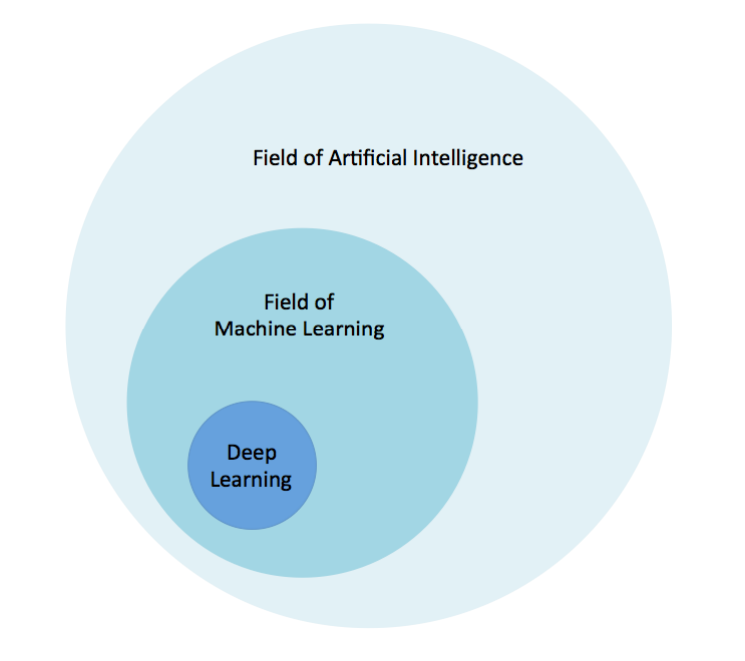
\includegraphics[width= 10cm]{../figuras/ia_ml.png}
  \caption{Relação entre inteligência artificial, \textit{machine learning} e aprendizado profundo (\citealt[][p.4]{dl-oreilly})}
  \label{fig:ia_ml}
\end{figure}

\section{Modelos de Aprendizado Automático}
 
Os modelos de \textit{machine learning} podem realizar várias categorias 
de tarefas, dentre elas a regressão e a classificação, a 
depender da atividade realizada pelo algoritmo. Os modelos de regressão têm como objetivo é prever um valor real a 
partir dos dados de entrada, segundo \citet{Goodfellow-et-al-2016}.
É possível, então, descrever cada entrada (\textit{input}) dos modelos como um vetor $x$ com 
$n$ atributos (\textit{features})\footnote{Neste estudo, 
os atributos utilizadas são indicadores econômicos, monetários,
sociais e da construção civil descritos na seção \ref{sec:dados}.} tal que
$x \in \mathbb{R}^n , x=\{x_1, x_2, ..., x_n\}$ e o 
processamento realizado pelos modelos de regressão com a função\footnote{As equações apresentadas neste subcapítulo foram retiradas de \cite{Goodfellow-et-al-2016}.} $ f : \mathbb{R}^n \rightarrow \mathbb{R}$. 

Os modelos de classificação, doutro modo, têm como objetivo 
determinar a qual das $k$ categorias disponíveis um 
\textit{input} pertence, conforme explica \citet{dl-oreilly}. Então, é utilizada uma função  
$ f : \mathbb{R}^n \rightarrow \{1,...,k\}$, quando 
$ f(x) = y$, o vetor de entrada $x$ foi classificado 
na categoria $y$. Um exemplo de tarefa de classificação
seria determinar se uma operação com cartão de crédito 
é fraudulenta ou não; neste trabalho, contudo, não foi empregado 
tal tipo de modelo, apenas modelos de regressão. 

Ainda conforme \citet{Goodfellow-et-al-2016}, os problemas de 
\textit{machine learning} também podem ser divididos entre
aprendizado não-supervisionado e supervisionado. No primeiro, 
o modelo recebe um conjunto de dados (\textit{dataset}) não 
rotulado e aprende propriedades de sua estrutura. 
Um exemplo de aprendizado não supervisionado é o \textit{clustering},
que consiste em dividir o conjunto de dados
em agrupamentos (\textit{clusters}) com amostras similares. No segundo, por outro lado, 
os dados de entrada estão associados a resultados conhecidos, 
chamados de \textit{labels} ou rótulos. Neste estudo, utiliza-se aprendizado 
supervisionado para prever o consumo de cimento mensal nos 
estados da União a partir dos dados de entrada e compará-los 
com o valor real 
do consumo e, assim, calcular a precisão do modelo.

\section{Modelos utilizados}

Para a produção desta pesquisa, foram utilizadas três categorias de modelos de \textit{machine learning} para prever a demanda por cimento: regressão linear, redes
neurais \textit{feed forward} e redes recorrentes. Foram testados, também,
 métodos de pré-processamento de dados\footnote{Os métodos de pré-processamento de dados são descritos na seção \ref{sec:norm_dados}.} e  diferentes arquiteturas de 
redes neurais ao alterar o número de camadas, a quantidade de neurônios
em cada camada, o tipo de camada, a função de ativação, entre outras
configurações, tudo isso com o objetivo de comparar 
o desempenho dos modelos e encontrar o que apresenta menor erro na previsão.

\subsection{Regressão linear}
\label{sec:reg_lin}

A regressão linear é um modelo de \textit{machine learning} que assume um relacionamento
linear entre a variável que será prevista (\textit{target}) e os dados de entrada, conforme explica \citet{forecasting}.
Desse modo, o intuito é construir uma 
função que, para cada par\footnote{No
caso deste estudo, o par  $(x,y)$ é tal que 
$x$ representa o valor de cada
indicador descrito na seção \ref{sec:dados} em um estado, mês e ano, enquanto 
$y$ corresponde ao número de toneladas de cimento consumidas
por esse estado nessa data.} $(x,y)$, recebe como
entrada o vetor $x$ correspondente às variáveis de \textit{input},
$x \in \mathbb{R}^k , x=\{x_1, x_2, ..., x_k\}$ e calcula coeficientes
$\beta = \{\beta_0, \beta_1, \dots, \beta_k\}$ para cada atributo de $x$,
além da constante $\beta_0$. O algoritmo, então, utiliza esses coeficientes para
prever o valor da variável \textit{target}, $y$, sendo 
que $y \in \mathbb{R}$. Seja,
então, $\hat{y}$ o valor previsto pelo modelo para um 
par $(x, y)$, a função que descreve a 
regressão linear, então, é dada pela equação \ref{eq:lse}:

\begin{equation}
  \hat{y} = f(x) = \beta_0 + \beta_1 x_{1_i} + \beta_2 x_{2_i} + \dots + \beta_k x_{k_i} 
  \label{eq:lse}
\end{equation}

Logo, é possível contruir uma matriz $X$ em que a linha $i$
corresponde ao vetor $x_i$ dos dados de entrada e 
cada coluna $j$ representa uma \textit{feature}. Pode-se, 
além disso, construir a matriz $\beta$ dos coeficientes associados 
a cada elemento da matriz $X$. Assim, o modelo
é dado por:

\begin{equation}
  \label{eq:reg_lin}
  y = X\beta + \epsilon
\end{equation}

Na equação \ref{eq:reg_lin}, $\epsilon$ é o vetor com o erro associado a cada umas 
das previsões; lembrando que $\epsilon_i$ é a i-ésima entrada do vetor $\epsilon$, assim como $\epsilon_i = y_i - \hat{y_i} = y - (\beta_0 + \beta_1 x_1 + \beta_2 x_2 + \dots + \beta_k x_k )$.
Os coeficientes $\beta$ são calculados durante o treinamento 
do modelo utilizando o método do \textit{least squares estimation},
que visa minimizar a soma do erro quadrado associado às previsões, 
como descrito em:

\begin{equation}
  \sum_{i=1}^{n} \epsilon_i^2 = \sum_{i=1}^{n} (y_i - \hat{y_i})^2 = 
  \sum_{i=1}^{n} (y_i - (\beta_0 + \beta_1 x_{1_i} + \beta_2 x_{2_i} + \dots + \beta_k x_{k_i} ))^2
\end{equation}

Os coeficientes $\beta_1, \beta_2, \dots, \beta_k$ 
determinam como cada atributo de entrada afeta a previsão, no presente caso, o consumo de cimento.
Por exemplo, se o coeficiente da variável $x_i$ for $\beta_i = 0$,
essa variável não terá influência no valor previsto pelo modelo. 
Caso o coeficiente seja positivo um aumento 
no valor de $x_i$ resultará no aumento do valor previsto $\hat{y_i}$,
já se $\beta_i$ for negativo, um aumento no valor de $x_i$  refletirá na 
diminuição no valor de $\hat{y_i}$. 


Na imagem \ref{fig:reg_lin}, há um exemplo de um modelo de regressão 
linear com apenas uma variável:

\begin{figure}[H] 
  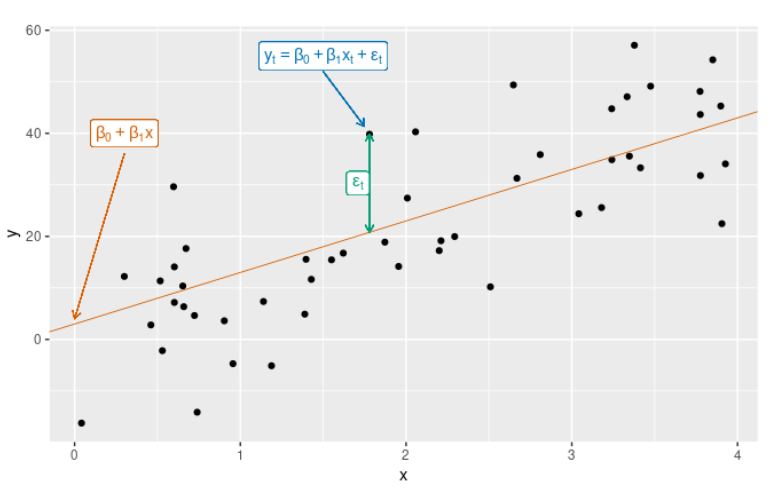
\includegraphics[width= 10cm]{../figuras/reg_lin.png}
  \caption{Exemplo de um modelo simples de regressão linear. Imagem retirada de \citet{forecasting} e disponível em \url{https://otexts.com/fpp3/regression-intro.html}}
  \label{fig:reg_lin}
\end{figure}

Na  figura \ref{fig:reg_lin}, as observações $y_i$ estão 
representadas pelos pontos pretos, enquanto a linha em laranja
corresponde à previsão realizada pelo modelo. Observa-se que
o modelo não prevê com total exatidão os dados observados, isso porque há 
um erro associado a cada previsão $-$ o que é um comportamento esperado, já que fenômenos previstos são 
sujeitos a fatores externos e não lineares $-$, como o destacado em verde 
na ilustração.


Por se tratar de um modelo mais simples, os resultados obtidos
com a regressão linear são utilizados neste trabalho como base 
para comparar o desempenho de modelos mais robustos.

\subsection{Redes neurais}

Redes neurais são modelos de \textit{machine learning} inspirados no funcionamento
do cérebro animal, formado por neurônios que se
conectam para transmitir informações sem a necessidade de 
controle central, segundo \citet{deeplearningbook} e \citet{dl-oreilly}. Um neurônio biológico, então, 
é uma célula nervosa que se comunica com outros neurônios 
por meio de impulsos eletroquímicos. Essa comunicação é 
denominada sinapse e ocorre apenas se o impulso 
for forte o bastante para ativar a liberação de
químicos na fenda sináptica. 

Um neurônio biológicoé composto por vários dendritos, 
um axônio e um corpo celular, como ilustrado na figura \ref{fig:neuron}:

\begin{figure}[H] 
  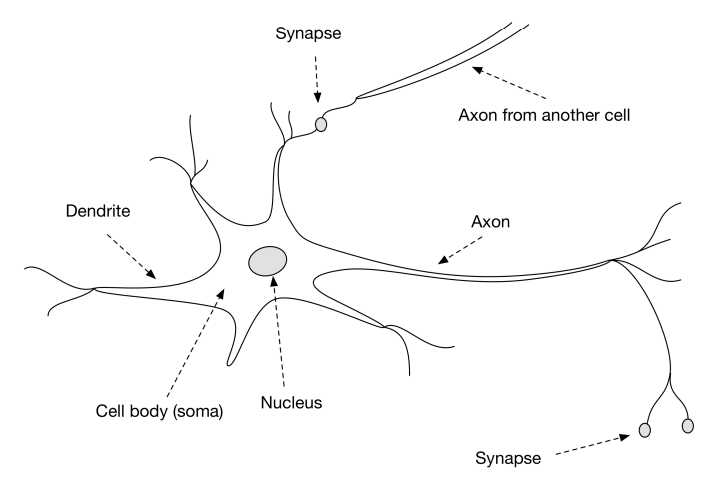
\includegraphics[width= 12cm]{../figuras/neuron.png}
  \caption{Ilustração de um neurônio biológico (\citealt[][p.44]{dl-oreilly})}
  \label{fig:neuron}
\end{figure}

Destaca-se na figura \ref{fig:neuron} a informação chegando a um 
dendrito do neurônio em destaque
por meio de uma sinapse, também está representada a comunicação com outra célula
por meio de outra sinapse iniciada no axônio 
do neurônio em questão. 

O processo de propagação da informação nos neurônios 
envolve as três partes da célula: dendritos, corpo celular
e axônio.
Os dendritos recebem informações de neurônios vizinhos 
na forma de impulsos elétricos e são responsáveis 
por conduzí-las até o corpo celular. 
Ao chegar ao local, a informação é processada, e novos 
impulsos são gerados e repassados a outro neurônio 
por meio do axônio no processo de sinapse, segundo \citet{fund_deep_learning} e  \citet{deeplearningbook}.
A estrutura e funcionamento dos neurônios biológicos inspiraram
os cientistas ao projetarem neurônios artificiais, como 
os \textit{perceptrons}. 

\subsubsection{Neurônios artificiais}

O \textit{perceptron} foi desenvolvido em 1957 por Frank 
Rosenblatt, inspirado nos trabalhos de Warren McCulloch e Walter Pitts\footnote{Em 
1943, Warren McCulloch e Walter Pitts apresentaram a 
primeira ideia de neurônio artificial.(\cite{neuronio})}.
Trata-se de um modelo linear de classificação que 
recebe $n$ entradas e produz uma saída binária, como mostrado 
na ilustração simplificada \ref{fig:perceptron-simples}. Ainda de acordo com \citet{deeplearningbook}, esse modelo inicial apresentava limitações e passou por evoluções com o passar do 
tempo. Apesar disso, as redes neurais atualmente utilizam, em geral,
outro modelo de neurônio, como o ilustrado na imagem \ref{fig:perceptron}:


\begin{figure}[H]  
  \centering
  \begin{subfigure}{7cm}
    \centering 
    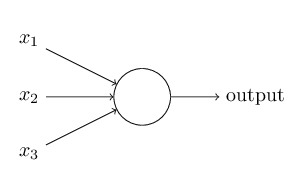
\includegraphics[width=7cm]{../figuras/perceptron-simples.png}
    \caption{Visão simplificada de um neurônio. Imagem retirada de \citet{deeplearningbook} e disponível em \url{https://www.deeplearningbook.com.br/o-perceptron-parte-1/}}
    \label{fig:perceptron-simples}
  \end{subfigure}
  \hfill
  \begin{subfigure}{7cm}
    \centering
    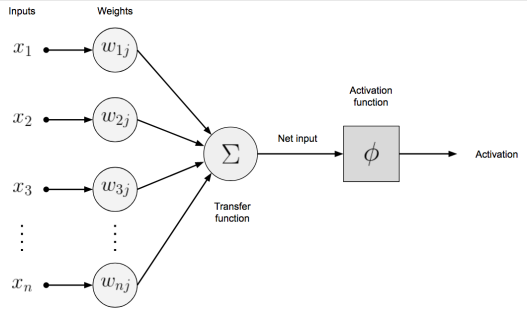
\includegraphics[width=7cm]{../figuras/perceptron.png}
    \caption{Ilustração da arquitetura de um 
    neurônio artificial (\citealt[][p.50]{dl-oreilly})}
    \label{fig:perceptron}
  \end{subfigure}
  \caption{Neurônios artificiais}
\end{figure}

A figura \ref{fig:perceptron} mostra o funcionamento de 
um neurônio artificial. O neurônio apresenta $n$ entradas 
$x_i$, cada uma associada a um peso $w_i$, que expressa 
a importância da respectiva entrada para o valor de saída\footnote{ 
O peso atribuído a uma das entradas expressa a influência
desta no \textit{output} do nó, de modo similar aos coeficientes calculados 
para cada atributo da regressão linear, explicada na seção \ref{sec:reg_lin}},
oproduto escalar entre os pesos e as respectivas entradas
 passa por uma função de 
ativação\footnote{Um detalhamento sobre as funções de 
ativação pode ser encontrado na subseção \ref{sec:funcao_ativacao}} 
$\phi$ que determina a saída do neurônio. 
Além disso, ainda segundo \citet{deeplearningbook} e \citet{dl-oreilly}, um valor de \textit{bias} ou polarização é
adicionado ao produto escalar e possibilita que 
um neurônio com todas as entradas nulas
apresente saída não nula, de modo a
aumentar a capacidade de aproximação da rede. 

% É possível, então, traçar um paralelo entre o neurônio
% artificial e o biológio. Em primeiro lugar, as entradas 
% $x_i$ do neurônio  têm um funcionamento similar aos 
% dentritos responsáveis 
% por receber as informações que chegam à celula. Em segundo lugar,
% o processamento matemático entre as entradas e os pesos 
% tem comportamento similar ao corpo 
% celular do neurônio biológico, que processa a informação 
% recebida. Por fim, a função de ativação é responsável por modelar o 
% \textit{output} que será repassado às camadas seguintes como uma das entradas
% assim como o neurônio repassa, por meio de sinapses, os impulsos processados
% a outros neurônios.


Seja $x$ o vetor das $n$ entradas do neurônio,
$x \in \mathbb{R}^n, x=\{x_1, x_2, ..., x_n\}$, e seja 
$w$ o vetor com os pesos associados a cada entrada, 
$w \in \mathbb{R}^n, w=\{w_1, w_2, ..., w_n\}$. Além disso,
seja $b$ o valor de \textit{bias} e $\phi$ a função de ativação.
Dessa forma, o \textit{output} $h$ de um neurônio é dado por:
 
\begin{equation}
  h_{w,b} = \phi(w \cdot x + b)
\end{equation}

Essa saída é utilizada como uma das entradas dos neurônios
na camada seguinte, de modo a formar a estrutura das redes 
neurais. 

Os neurônios,
então, formam a unidade que compõe as redes neurais artificiais,
como ilustrado na figura \ref{fig:redeneural}:

\begin{figure}[H] 
  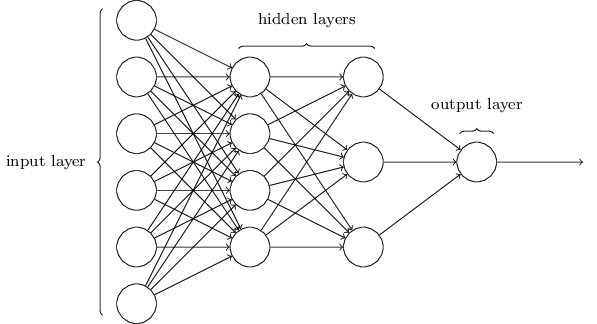
\includegraphics[width= 12cm]{../figuras/redes/rede_mlp.png}
  \caption{Ilustração de uma rede neural obtida de 
  \citet{neuralnetworksanddeeplearning}} 
  \label{fig:redeneural}
\end{figure}

A imagem \ref{fig:redeneural} representa uma simplificação de uma 
rede neural. A informação chega a uma camada da rede, é processada pelo neurônios e repassada para a camada seguinte, até obter a saída final. Em particular, é representada uma
rede \textit{feed forward}, uma vez que não há conexões entre neurônios de uma 
mesma camada nem conexões entre uma camada e a anterior. A informação então 
se propaga apenas no sentido da camada de entrada em direção à final, de saída.


Além disso, em \ref{fig:redeneural}, é ilustrada uma rede neural \textit{feed forward}.
Conforme a figura, a camada mais à esquerda da rede é 
denomida \textit{input layer}, a camada mais à direita, de \textit{output layer},
e as camadas intermediárias são chamadas \textit{hidden layers}.
Por razões históricas, de acordo com \citet{neuralnetworksanddeeplearning}, é possível encontrar referências a essas redes como
\textit{multilayer perceptron}, contudo, as redes em geral
utilizam neurônios sigmóides ao invés de \textit{perceptrons}.

\subsubsection{Função de ativação}
\label{sec:funcao_ativacao}

A função de ativação determina se um neurônio será ativado, ou seja, 
se a saída será propagada para a camada seguinte. Enquanto os pesos 
e o \textit{bias} realizam uma transformação linear nos dados 
de entrada, a função de ativação aplica uma transformação não
linear, assim, possibilita que a rede neural resolva
problemas não lineares e complexos, como reconhecer padrões de 
escrita, de acordo com \citet{deeplearningbook} e \citet{zhang2021dive}. 

A função de ativação é um atributo de cada uma das camadas 
da rede e é escolhida de acordo com a tarefa que será 
executada. Por exemplo, a função sigmóide é recomendada
 para problemas de classificação. Neste estudo, 
foram utilizadas as funções \textit{rectified linear unit} (ReLU) e \textit{swish}.

\subsubsection{\textit{Rectified linear unit} (ReLU)}

A função ReLU, do inglês \textit{rectified linear unit}, é a
função de ativação mais popular atualmente, uma vez que apresenta bom desempenho 
em diferentes tarefas, conforme \citet{dl-oreilly}. A função ReLU é dada por:

\begin{equation}
  f(x) = max(0,x)
\end{equation}

Ainda segundo \citet{dl-oreilly}, por possuir derivada igual a zero ou a uma constante, a ReLU não sofre do problema da dissipação do gradiente\footnote{Um 
detalhamento sobre o problema da dissipação do gradiente será dado na subseção \ref{sec:vanishing_gradient_problem}.} como
outras funções de ativação, 
uma vez que a derivada é utilizada nos modelos de \textit{machine learning}
para atualizar os pesos e \textit{bias} no treinamento da rede.
O gráfico da função ReLU está ilustrado na figura \ref{fig:relu}:

\begin{figure}[H] 
  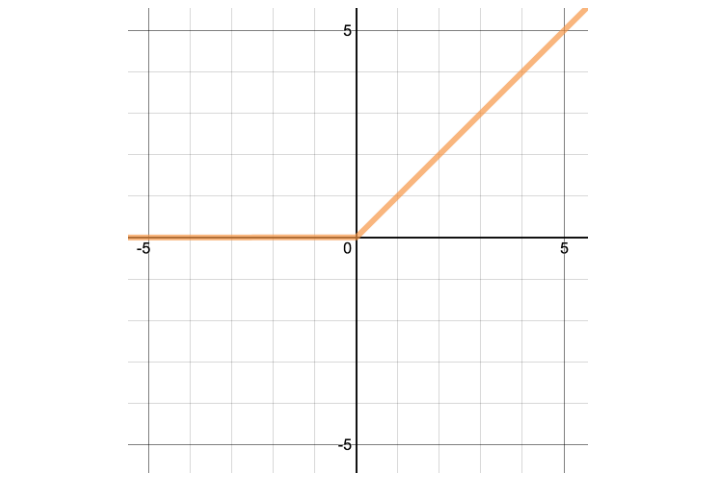
\includegraphics[width= 8cm]{../figuras/relu.png}
  \caption{Rectified linear unit (ReLU) (\cite{dl-oreilly})}
  \label{fig:relu}
\end{figure}

\subsubsection{Swish}

A função \textit{swish} foi proposta por pesquisadores da 
Google em 2017, com a promessa de apresentar desempenho igual 
ou superior à ReLU em redes neurais profundas, conforme \cite{swish}. A \textit{swish} é uma função 
não monótona\footnote{Uma função definida como $f: I \rightarrow \mathbb{R}$
é monótona se é não crescente no intervalo $I$ ou não decrescente em $I$.} e 
suave\footnote{Uma função $f$ é suave se possui derivada de todas as ordens.},
cuja fórmula é dada por:

\begin{equation}
  f(x) = x \cdot sigmoid(x) = \frac{x}{1+e^{-x}}
\end{equation}


O gráfico da função é similar ao da ReLU e pode ser observado na imagem \ref{fig:swish}:

\begin{figure}[H] 
  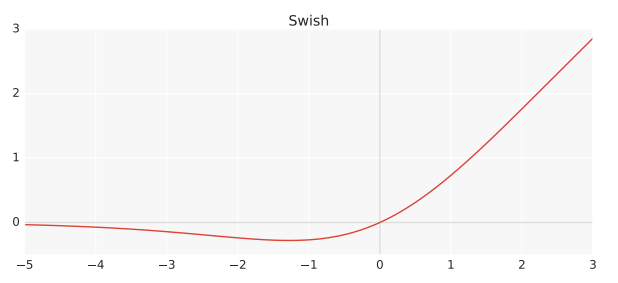
\includegraphics[width= 12cm]{../figuras/swish.png}
  \caption{Função \textit{swish} (\cite{swish})}
  \label{fig:swish}
\end{figure}


\subsubsection{Problema da Dissipação do Gradiente}
\label{sec:vanishing_gradient_problem}

O aprendizado de uma rede neural ocorre ao alterar os valores dos pesos
e \textit{bias} dos neurônios de acordo com a função de custo ou \textit{loss function} (\cite{neuralnetworksanddeeplearning}). 
Sejam $x$, $w$ e $b$ os conjuntos de entradas,
pesos e \textit{bias} da rede, respectivamente. Então, a função de custo $C$ é dada por:

\begin{equation}
  C(w,b) = \frac{1}{2n}\sum_x || y(x) - a ||^2
\label{eq:func_custo}
\end{equation}

Na equação acima, $y(x)$ representa o vetor com as respostas
que a rede tenta prever, $a$ é o vetor de \textit{output} da rede e 
$n$ é o número total de entradas de treino. Assim, é possível calcular o gradiente $\delta_j^i$
relativo ao $j$-ésimo neurônio da $i$-ésima camada:

\begin{equation}
  \delta_j^i = \frac{\partial C}{\partial b_j^i}
\label{eq:func_grad}
\end{equation}

Seja $\delta^i$ o vetor cujos elementos estão associados
aos neurônios da camada $i$. Como os gradientes definem a alteração nos pesos 
e \textit{bias}
de cada neurônio,  $\delta^i$  determina a velocidade de aprendizado dessa camada.

O problema da dissipação do gradiente\footnote{O problema da dissipação do gradiente 
é conhecido em inglês como \textit{the vanishing gradient problem}.
}, de acordo com \citet{deeplearningbook}, ocorre quando os gradientes das camadas iniciais ficam com valores 
muito próximos a zero e atinge, em especial, modelos 
de \textit{deep learning} com muitas camadas e redes recorrente. Por conta disso, os pesos e \textit{bias} não são atualizados
de forma eficiente nessas camadas, de tal forma que o treinamento e aprendizado
tornam-se demasiadamente lentos. 
        
\subsection{Redes neurais recorrentes}
\label{rnn}

Redes recorrentes são uma subclasse das redes neurais e possuem a capacidade
de capturar o contexto como diferencial frente às redes \textit{feed forward}
tradicionais. Por levar em consideração o presente e o passado recente ao 
realizar uma previsão, apresentam bom desempenho na previsão de séries 
temporais ou sequências. Há várias implementações possíveis de redes 
recorrentes. Neste trabalho testaram-se as redes LSTM e GRU.

\subsubsection{Redes LSTM}

As redes \textit{Long Short Term Memory} (LSTM) foram introduzidas em 1997 por Hochreiter 
e Schmidhuber\footnote{As redes neurais LSTM foram apresentadas no artigo \cite{lstm-origem}.}.
Atualmente, são a variação mais utilizada de redes
neurais recorrentes, em particular, na classificação de séries temporais e
reconhecimento de fala. Segundo \citet{deeplearningbook}, redes LSTM apresentam células de 
memória conectadas cujo conteúdo é modulado pelo \textit{input gate} e o \textit{forget gate}\footnote{Um 
melhor detalhamento sobre o \textit{input gate} e o \textit{forget gate} será 
dado mais adiante nesta seção.}.
Por exemplo, se ambos estiverem fechados em um instante, o conteúdo da célula permanecerá 
o mesmo no instante em questão e no próximo. Essa estrutura permite que a informação
seja retida ao longo do tempo e evita o problema do \textit{vanishing gradient} que 
ocorre com a maioria das redes recorrentes.

As redes neurais LSTM apresentam uma arquitetura diferente 
das redes tradicionais, uma vez que há ciclos de \textit{feedback}
nas conexões entre as células. Para melhor ilustrar essa 
arquitetura, \cite{dl-oreilly} utilizam a visualização \textit{flat} 
 (achatada) das redes neurais, na qual as células de uma mesma 
camada da rede estão representadas como um único nó.
Pode-se observar essa representação em uma rede tradicional 
\textit{feed forward}
na imagem \ref{fig:arq-ff-flat} e, em
\ref{fig:arq-ff}, a representação 
tradicional:

\begin{figure}[H]
  \centering
  \begin{subfigure}{7.5cm}
      \centering
      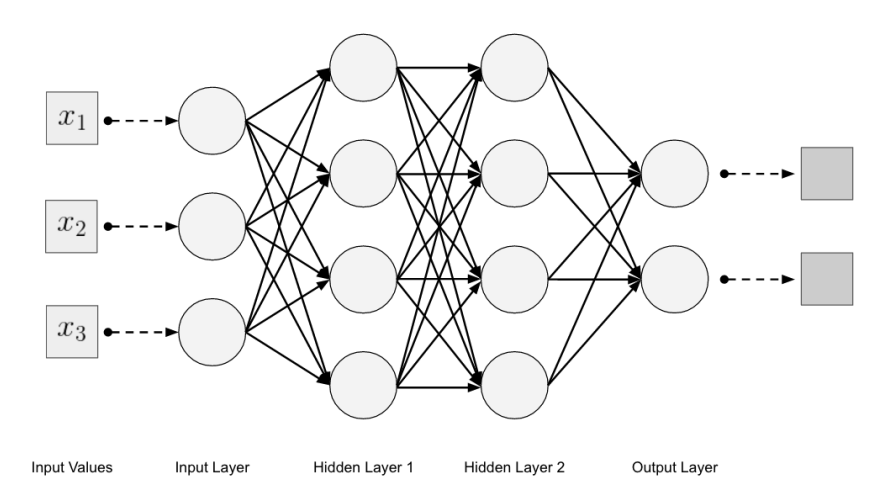
\includegraphics[width=7.5cm]{../figuras/redes/arq-ff.png}
      \caption{Arquitetura de rede neural \textit{feed forward}}
      \label{fig:arq-ff}
  \end{subfigure}
  \hfill
  \begin{subfigure}{7.5cm}
      \centering
      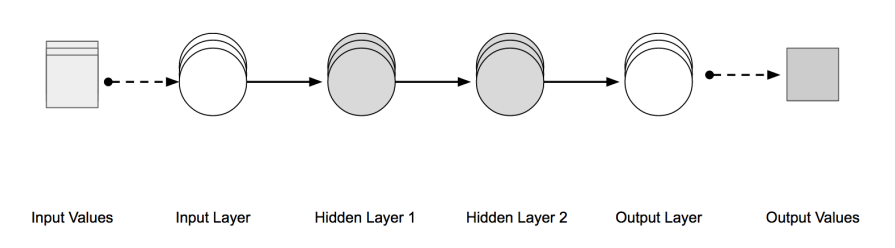
\includegraphics[width=7.5cm]{../figuras/redes/arq-ff-flat.png}
      \caption{Visão \textit{flat} (achatada) da arquitetura de uma rede neural \textit{feed forward} }
      \label{fig:arq-ff-flat}
  \end{subfigure}
  \label{fig:comparacao-ff-flat-normal}
  \caption{Arquitetura de uma rede \textit{feed forward}}
\end{figure}

As redes LSTM introduzem o conceito de conexão entre a saída de uma 
camada oculta da rede neural e a entrada da mesma camada. A partir desse
ciclo, obtém-se \textit{outputs} de tempos anteriores como parte da informação que 
chega ao tempo atual. Na figura \ref{fig:arq-rnn-flat}, essas 
conexões recorrentes são representadas como as setas que saem de uma célula e 
atingem a mesma célula, uma vez que se utiliza a representação achatada.
A imagem \ref{fig:arq-rnnff}, por sua vez, representa a rede LSTM desenrolada 
atráves do eixo do tempo:

\begin{figure}[H]
  \centering
  \begin{subfigure}{7.5cm}
      \centering
      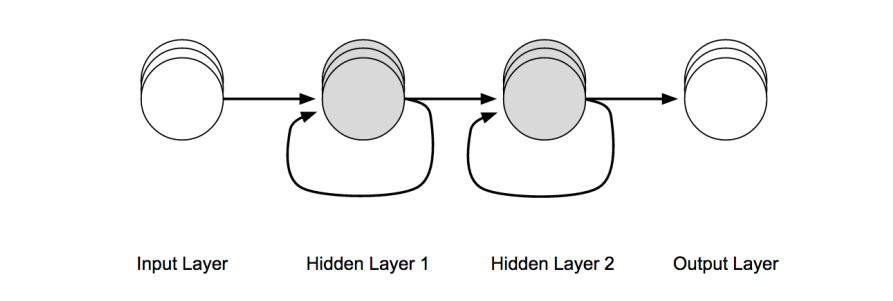
\includegraphics[width=7.5cm]{../figuras/redes/arq-rnn-flat.png}
      \caption{Visão \textit{flat} (achatada) arquitetura de rede neural LSTM }
      \label{fig:arq-rnn-flat}
  \end{subfigure}
  \begin{subfigure}{7.5cm}
    \centering
    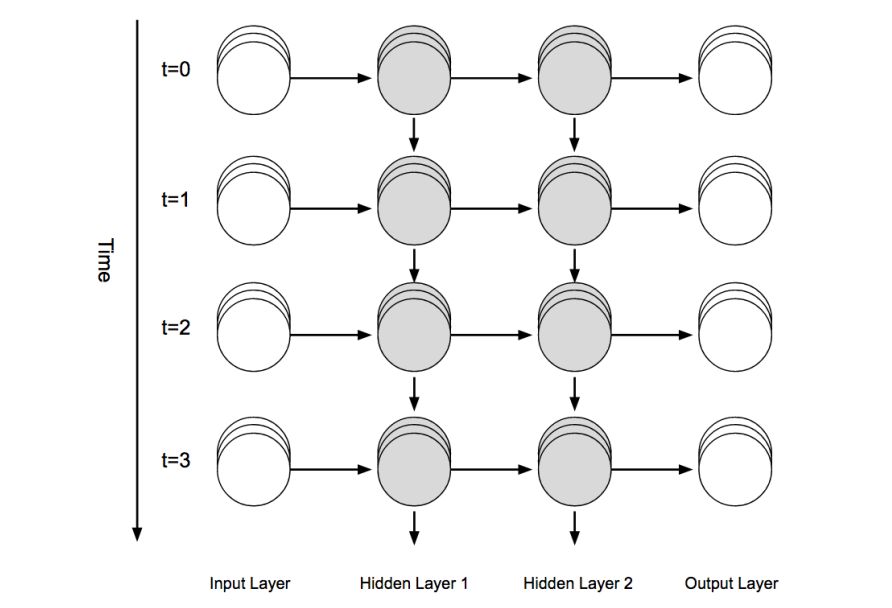
\includegraphics[width=7.5cm]{../figuras/redes/arq-rnn.png}
    \caption{Visão da rede neural LSTM ao longo do tempo}
    \label{fig:arq-rnnff}
  \end{subfigure}
  \hfill
  \label{fig:comparacao-rnn-flat-normal}
  \caption{Arquitetura das redes recorrentes}
\end{figure}

As unidades que formam cada uma das camadas de uma LSTM são uma variação dos
neurônios artificiais clássicos. Essas unidades, representadas em \ref{fig:lstm-cell},
 permitem que a rede mantenha o estado
ao longo do tempo e apresentam conexões vindas da camada anterior e de \textit{outputs} 
dessa
mesma unidade em tempos anteriores:

\begin{figure}[H]
  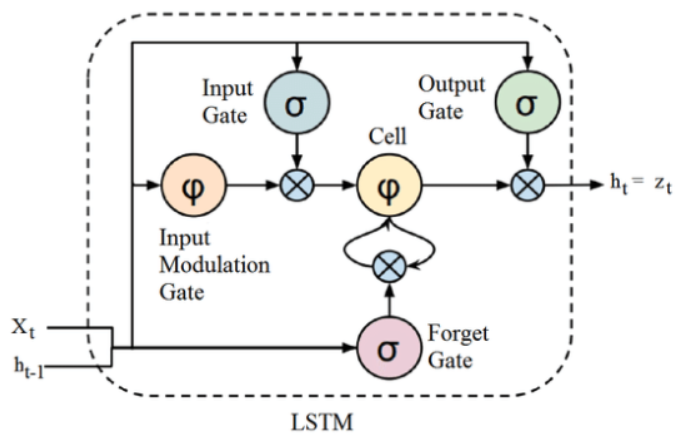
\includegraphics[width=9cm]{../figuras/redes/lstm-cell.png}
  \caption{Célula de memória de rede LSTM (\cite{deeplearningbook})}
  \label{fig:lstm-cell}
\end{figure}

A unidade LSTM recebe duas entradas: a observação no tempo atual e a saída do 
último estado oculto. Nela, a informação é retida nas células e as manipulações de memória 
são realizadas nos \textit{gates} (portões). O \textit{forget gate} é responsável
por remover informações que não são mais úteis para a célula, ou seja, pelo 
esquecimento. Essa operação é realizada por meio de multiplicação de matrizes 
de pesos, adição de parâmetro de viés e aplicação de uma função de ativação que fornece uma saída binária. 
O \textit{input gate}, por sua vez, adiciona informações úteis ao estado da célula
a partir da aplicação de funções sigmóides e tangente hiperbólica, além da multiplicação de vetores. 
Por fim, o \textit{output gate} extrai informações úteis ao estado da célula atual 
para apresentar como saída da célula e entrada para a seguinte, com o auxílio de funções tangente
hiperbólica e sigmoide, além da multiplicação de vetores. (\cite{deeplearningbook})

\subsubsection{Redes GRU}


As redes \textit{gated recurrent units} são redes recorrentes
similares às LSTM e foram introduzidas por (\cite{gru}).
As unidades
das redes LSTM apresentam dois estados passados entre as células:
um que carrega memória de longo prazo e outro, de curto prazo. As unidades 
GRU, por sua vez, apresentam apenas um 
estado oculto carregado ao longo do tempo, capaz de manter
as dependências de curto e longo prazo (\cite{deeplearningbook}). A 
estrutura das unidades GRU pode ser vista em \ref{fig:gru-cell}:

\begin{figure}[H]
  \centering
  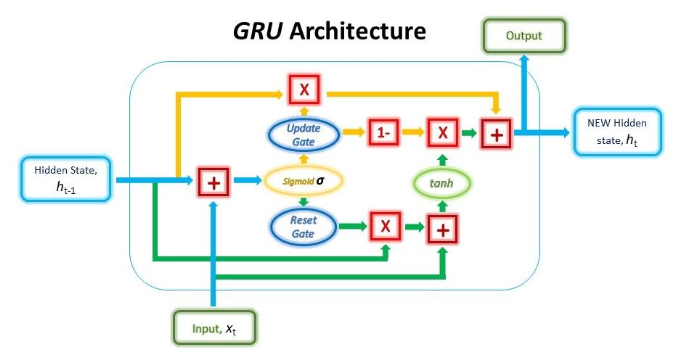
\includegraphics[width=9cm]{../figuras/redes/gru-cell.png}
  \caption{Unidade da rede GRU (\cite{deeplearningbook})}
  \label{fig:gru-cell}
\end{figure}

As unidades GRU apresentam portões, assim como as unidades LSTM,
para controlar o fluxo de informações. O \textit{reset gate}, ou
portão de redefinição, é responsável por controlar quais informações 
das etapas anteriores serão mantidas na etapa atual, por meio 
da função sigmoide e multiplicação de vetores. O \textit{update gate},
por sua vez, tem como objetivo determinar quanto das informações
armazenadas no estado oculto atual são apenas cópias do estado anterior. (\cite{d2l})

Por possuírem arquitetura mais simples, as redes GRU 
apresentam um treinamento mais rápido que as LSTM.

\subsection{Redes bidirecionais}

As redes bidirecionais foram introduzidas em 1997 por Schuster e Paliwal com a 
proposta de utilizar uma entrada para influenciar ao mesmo tempo as previsões 
do futuro e do passado (\cite{brnn}).
Redes recorrentes, como as LSTM e GRU, analisam uma entrada com base nos 
eventos passados e presentes. As redes bidirecionais, por outro lado, inovam ao 
considerar o passado, presente e o futuro ao realizar uma previsão. Por isso, 
apresentam bom desempenho em atividades como reconhecimento de escrita a mão, reconhecimento de
fala, processamento de linguagem natural. (\cite{bidirectional})

As redes bidirecionais combinam duas redes recorrentes para realizar a previsão. 
Uma rede analisa a sequência $x^{(i)}$
fornecida no \textit{input} do início $x_0$ em direção ao final $x_i$, a outra é treinada
no sentido oposto. As redes utilizadas podem ser simples redes 
recorrentes, redes LSTM ou GRU. Na figura \ref{fig:bi}, pode-se observar o 
treinamento das redes nos dois sentidos ocorrendo simultaneamente:

\begin{figure}[H]
  \centering
  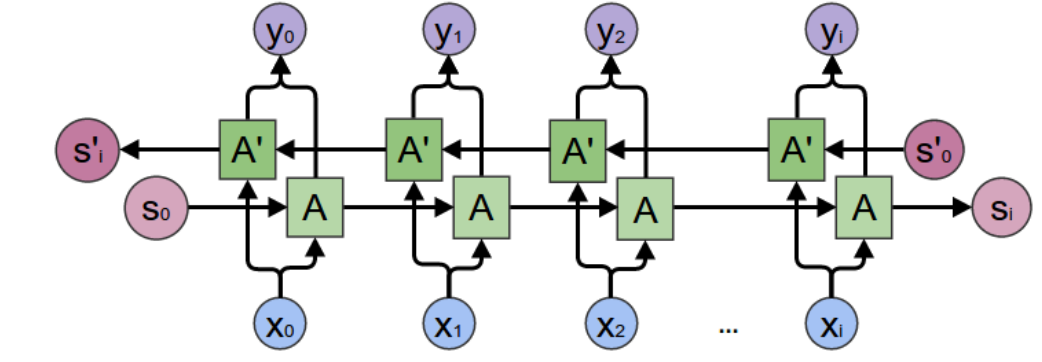
\includegraphics[width=9cm]{../figuras/redes/bi.png}
  \caption{Estrutura de rede bidirecional (\cite{bidirectional})}
  \label{fig:bi}
\end{figure}
